\chapter{Аутентификация и Авторизация}\label{chap:auth}

Аутентификация и авторизация две очень связанные, но в то же время различные концепции. В то время как первая имеет дело с идентификацией пользователя, вторая определяет, что пользователю позволенно делать. К сожалению, поскольку для обоих терминов часто используется абревиатура "auth", эти концепции часто объединяются.

Yesod обеспечивает встроенную поддержку для нескольких сторонних систем аутентификации, таки как OpenID, BrowserID и OAuth. Это внешние системы которым ваше приложение доверяет удостоверение личности пользователя. Также есть поддержка для более обычных систем аутентификации, таких как имя пользователя/пароль или адрес почты/пароль. Первый способ гарантирует простоту как для пользователей (нет неоходимости запоминать новые пароли), так и для разработчиков (нет нужды иметь дело со всей архитектурой безопасности), в то время как последний дает разработчику больший контроль.

Для авторизации, мы можем воспользоваться преймуществами REST и типобезопасными URL, чтобы создать простую, декларативную систему. К тому же, поскольку весь код авторизации написан на Haskell в вашем распоряжении будет вся гибкость языка.

В этой главе мы рассмотрим, как установить настроить "auth" решение в Yesod, и обсудим некоторые компромисы в различных опциях аутентификации.

\section{Обзор}

Пакет \footnotehref{http://hackage.haskell.org/package/yesod-auth}{yesod-auth} обеспечивает унифицированный интерефейс для различных плагинов аутентификации. Единственное что от требование для них, это чтобы они идентифицировали пользователя по какой-то уникальной строке. В OpenID, к примеру, это может быть фактическое значение OpenID. В BrowserID, это адрес электронной почты. Для HashDB (которая использует базу данных хэшированных паролей), это имя пользователя.

Каждый плагин аутентификации обеспечивает свою собственную систему для входа, либо через передачу токенов с внешнего сайта, или через форму адрес почты/пароль. После успешного входа, плагин устанавливает значение в пользовательской сессии, указывающее его \lstinline'AuthId'. Этот \lstinline'AuthId' это обычно Persistent ID из таблицы используемой для отслеживания пользователей. 

Есть несколько функций, доступные для запроса пользовательского \lstinline'AuthId', наиболее часто \lstinline'maybeAuthId', \lstinline'requireAuthId', \lstinline'maybeAuth' и \lstinline'requireAuth'. Версии require* перенаправляют на страницу входа, если пользователь ешё не вошел, а те функции, что не оканчиваются на Id, возвращают два значения --- ID таблицы и значение сущности.

Поскольку всё хранилище \lstinline'AuthId' построено на сессиях, то применимы все их правила. В часности, данные сохраняются зашифрованными, подписаное HMAC куки, который автоматически устаревает после определенного сконфигурированного периода неактивности. А также, поскольку не существует компоненты сессий на стороне сервера, при выходе из системы просто удаляются данные из куки сессии; если пользователь использует старое значение куки, сессия будет оставаться действительной.

\begin{remark}
В будущем мы планируем добавить к сессиям серверную часть, которая будет позволять делать принудительный выход пользователя. Почти точно это будет реализовано до релиза Yesod 1.0.
\end{remark}

С другой стороны, авторизация обрабатывается несколькими методами внутри класса типов \lstinline'Yesod'. Эти методы запускаются для каждого запроса, что бы определить, должен ли доступ быть разрешен, запрещен, или необходимо чтобы пользователь был авторизован. По умолчанию, эти метода разрешают доступ для каждого запроса. В качестве альтернативы, вы можете реализовать авторизацию более специальном способом, добавив вызовы \lstinline'requireAuth' и подобных функций в индивидуальных функциях обработчиках, хотя это убирает преймущества декларативной системы авторизации.

\section{Опознай меня}

Давайте сразу рассмотрим пример с аутентификацией.

\begin{lstlisting}
{-# LANGUAGE OverloadedStrings, TemplateHaskell, TypeFamilies,
             MultiParamTypeClasses, QuasiQuotes #-}
import Yesod
import Yesod.Auth
import Yesod.Auth.BrowserId
import Yesod.Auth.GoogleEmail
import Data.Text (Text)
import Network.HTTP.Conduit (Manager, newManager, def)

data MyAuthSite = MyAuthSite
    { httpManager :: Manager
    }

mkYesod "MyAuthSite" [parseRoutes|
/ RootR GET
/auth AuthR Auth getAuth
|]

instance Yesod MyAuthSite where
    -- Внимание! Что бы работал вход с BrowserID, вы должны здесь
    -- корректно установить адрес вашего хоста.
    approot = ApprootStatic "http://localhost:3000"

instance YesodAuth MyAuthSite where
    type AuthId MyAuthSite = Text
    getAuthId = return . Just . credsIdent

    loginDest _ = RootR
    logoutDest _ = RootR

    authPlugins _ =
        [ authBrowserId
        , authGoogleEmail
        ]

    authHttpManager = httpManager

instance RenderMessage MyAuthSite FormMessage where
    renderMessage _ _ = defaultFormMessage

getRootR :: Handler RepHtml
getRootR = do
    maid <- maybeAuthId
    defaultLayout [whamlet|
<p>Your current auth ID: #{show maid}
$maybe _ <- maid
    <p>
        <a href=@{AuthR LogoutR}>Logout
$nothing
    <p>
        <a href=@{AuthR LoginR}>Go to the login page
|]

main :: IO ()
main = do
    man <- newManager def
    warpDebug 3000 $ MyAuthSite man
\end{lstlisting}

Мы начали с объявлений маршрута. Сперва объявили наш стандартный маршрут \lstinline'RootR', а затем определили подсайт для аутентификации. Запомните что ему нужны четыре параметра: путь к подсайту, имя маршрута, имя подсайта, и функция для получения значения подсайта. Другими словами, основываясь на строке:

\begin{lstlisting}
/auth AuthR Auth getAuth
\end{lstlisting}

Нам нужно иметь \lstinline'getAuth :: MyAuthSite -> Auth'. Пока мы ещё не написали эту функцию сами, \footnotehref{http://hackage.haskell.org/package/yesod-auth}{yesod-auth} предоставляет её автоматически. Для других подсайтов (к примеру со статическими файлами), мы обеспечиваем настройки конфигурации в значении подсайта, и вледствии этого нужно указать функцию get. Для подсайта auth, мы указываем эти настройки в отдельном классе типов, \lstinline'YesodAuth'.

\begin{remark}
Почему не использовать значение подсайта? Существует достаточно много настроек, которые мы бы хотели настраивать у auth подсайта, и делать это из типа записи (record type) было бы неудобно. Также, поскольку мы хотим иметь ассоциируемый тип \lstinline'AuthId', класс типов будет более естественным.

С другой стороны, почему не использовать класс типов для всех подсайтов? У этого есть минус: вы сможете иметь только один экземпляр класса на сайт, не позволяя раздавать различные наборы статичных файлов с различных маршрутов. Также, значение подсайта работает лучше если мы хотим загружать данные во время иницииализации приложения.
\end{remark}

Так что точно входит в экземпляр класса \lstinline'YesodAuth'? Есть шесть необходимых объявлений:

\begin{itemize}
    \item \lstinline'AuthId' это ассоциированный тип. Это то значение которое \lstinline'yesod-auth' будет давать вам когда вы будете спрашивать, вошёл ли пользователь (через \lstinline'maybeAuthId' или \lstinline'requireAuthId'). В нашем случае, мы просто используем \lstinline'Text', для сохранения необработанного идентификатора --- в нашем случае адреса электронной почты, как мы скоро увидим. 

    \item \lstinline'getAuthId' получает текущий \lstinline'AuthId' из типа данных \lstinline'Creds' (credentials --- учетные данные). Этот тип имеет три части информации: используемый способ аутентификации (в нашем случае browserid или googleemail), текущий идентификатор, и ассоциированный список с различной дополнительной информацией.

    \item \lstinline'loginDest' возвращает маршрут куда перенаправить пользователя после успешного входа.

    \item Подобно, \lstinline'logoutDest' возвращает маршрут для перенаправления после выхода. 

    \item \lstinline'authPlugins' это список используемых способов аутентификации. В нашем примере, мы используем BrowserID, который входит через систему Mozilla BrowserID, и Google Email, который аутентифицирует пользовательский почтовый адрес используя его Google аккаунт. Что хорошо в этих двух способах это:
    
    \begin{itemize}
        \item Они не требуют предустановки, в отличие от Facebook или OAuth, которые требуют установки учетных данных.
        
        \item Они используют адрес электронной почты как идентификатор, что людям более комфортно, в отличие от OpenID, которые используют URL. 
    \end{itemize}
    
    \item \lstinline'authHttpManager' получает менеджер соединений HTTP из основного типа. Это позволяет системам аутентификации, которые использует HTTP соединения (то есть почти все сторонние системы входа), использовать их повторно, избегая стоимости установки нового TCP соединения для каждого запроса.
\end{itemize}

Наш обработчик \lstinline'RootR', содержит ссылки на страницы входа и выхода, зависящие от того зашёл пользователь или нет. Обратите внимание как мы конструируем эти ссылки на подсайт: первым идёт имя маршрута подсайта (\lstinline'AuthR'), а следом маршрут в подсайте (\lstinline'LoginR' и \lstinline'LogoutR').

Илюстрации ниже показывает процесс входа со стороны пользователя.

\begin{figure}[tbh]
  \centering
  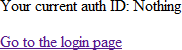
\includegraphics{14-initial-screen.png}
  \caption{Начальная загрузка страницы}
\end{figure}

\begin{figure}[tbh]
  \centering
  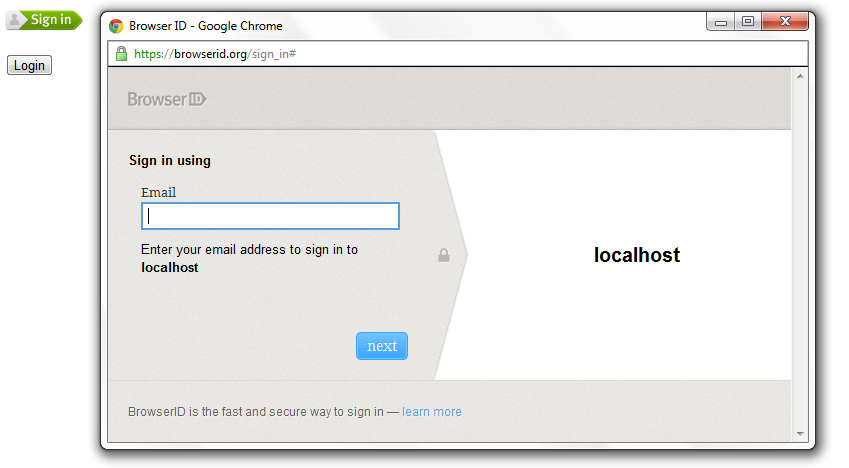
\includegraphics{14-login-with-browserid.png}
  \caption{Экран входа с помощью BrowserID}
\end{figure}

\begin{figure}[tbh]
  \centering
  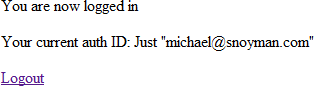
\includegraphics{14-after-login.png}
  \caption{Домащняя страница после входа}
\end{figure}

\section{Электронная почта}

Для большинства случаев будет достаточно аутентификации по адресу электронной почты. Иногда, вам может понадобиться чтобы пользователи использовали пароль для вашего сайта. Сгенерированый сайт не включает это, потому что:

\begin{itemize}
    \item Что бы безопасно использовать пароль, надо ипользовать SSL. Многие не предоставляют доступ к сайту по SSL.

    \item В то время как системы аутентификации по адресу электронной почты должным образом хранят пароли, скомпрометировнная база данных может быть проблемой. Мы не делаем никаких предположений, что пользователи Yesod следуют практике безопасной разработки.

    \item Вам нужна работающая система для посылки электронной почты. Много веб серверов в наши дни не справляются со всеми механизмами защиты от спама используемыми почтовыми серверами.

    \begin{remark}
    Пример ниже использует системную программу для отправки писем --- sendmail (только Unix). Если вы захотите избежать хлопот работая с серверами электронной почты самостоятельно, вы можете использовать Amazon SES. Есть пакет \footnotehref{http://hackage.haskell.org/package/mime-mail-ses}{mime-mail-ses}, который обеспечивает альтернативу использованию sendmail. Этот подход мы используем на сайте Haskellers.com.
    \end{remark}
\end{itemize}

Но допустим, что вам понадобиться иметь вход с паролем специфичным для вашего сайта. Для этого Yesod предоставляет встроенную реализацию. Для её использования от вас потребуется немного кода, ведь будет необходимо безопасно сохраненять пароли в базе данных, и отправлять пользователю несколько почтовых сообщений (проверка аккаунта, восстановление пароля, и т.д.).

Давайте посмотри на сайт предоставляющий аутентификацию по адресу электронной почты и паролю, хранящий пароли в Persistent SQLite базе данных.

\begin{lstlisting}
{-# LANGUAGE OverloadedStrings, TypeFamilies, QuasiQuotes, GADTs,
             TemplateHaskell, MultiParamTypeClasses, FlexibleContexts #-}
import Yesod
import Yesod.Auth
import Yesod.Auth.Email
import Database.Persist.Sqlite
import Database.Persist.TH
import Data.Text (Text)
import Network.Mail.Mime
import qualified Data.Text.Lazy.Encoding
import Text.Shakespeare.Text (stext)
import Text.Blaze.Html.Renderer.Utf8 (renderHtml)
import Text.Hamlet (shamlet)
import Data.Maybe (isJust)
import Control.Monad (join)

share [mkPersist sqlSettings, mkMigrate "migrateAll"] [persist|
User
    email Text
    password Text Maybe -- Пароль может быть ещё не задан
    verkey Text Maybe -- Используется для сброса пароля
    verified Bool
    UniqueUser email
|]

data MyEmailApp = MyEmailApp Connection

mkYesod "MyEmailApp" [parseRoutes|
/ RootR GET
/auth AuthR Auth getAuth
|]

instance Yesod MyEmailApp where
    -- Электронные письма будут содержать ссылки, так что убедитесь что включили approot, 
    -- что бы ссылки были правильными!
    approot = ApprootStatic "http://localhost:3000"

instance RenderMessage MyEmailApp FormMessage where
    renderMessage _ _ = defaultFormMessage

-- Установка Persistent
instance YesodPersist MyEmailApp where
    type YesodPersistBackend MyEmailApp = SqlPersist
    runDB f = do
        MyEmailApp conn <- getYesod
        runSqlConn f conn

instance YesodAuth MyEmailApp where
    type AuthId MyEmailApp = UserId

    loginDest _ = RootR
    logoutDest _ = RootR
    authPlugins _ = [authEmail]

    -- Необходимо найти UserId по заданному адресу электронной почты.
    getAuthId creds = runDB $ do
        x <- insertBy $ User (credsIdent creds) Nothing Nothing False
        return $ Just $
            case x of
                Left (Entity userid _) -> userid -- свеже добавленый пользователь
                Right userid -> userid -- существующий пользователь

    authHttpManager = error "Email doesn't need an HTTP manager"

-- Здесь весь код работающий с электронной почтой
instance YesodAuthEmail MyEmailApp where
    type AuthEmailId MyEmailApp = UserId

    addUnverified email verkey =
        runDB $ insert $ User email Nothing (Just verkey) False

    sendVerifyEmail email _ verurl =
        liftIO $ renderSendMail (emptyMail $ Address Nothing "noreply")
            { mailTo = [Address Nothing email]
            , mailHeaders =
                [ ("Subject", "Verify your email address")
                ]
            , mailParts = [[textPart, htmlPart]]
            }
      where
        textPart = Part
            { partType = "text/plain; charset=utf-8"
            , partEncoding = None
            , partFilename = Nothing
            , partContent = Data.Text.Lazy.Encoding.encodeUtf8 [stext|
Please confirm your email address by clicking on the link below.

\#{verurl}

Thank you
|]
            , partHeaders = []
            }
        htmlPart = Part
            { partType = "text/html; charset=utf-8"
            , partEncoding = None
            , partFilename = Nothing
            , partContent = renderHtml [shamlet|
<p>Please confirm your email address by clicking on the link below.
<p>
    <a href=#{verurl}>#{verurl}
<p>Thank you
|]
            , partHeaders = []
            }
    getVerifyKey = runDB . fmap (join . fmap userVerkey) . get
    setVerifyKey uid key = runDB $ update uid [UserVerkey =. Just key]
    verifyAccount uid = runDB $ do
        mu <- get uid
        case mu of
            Nothing -> return Nothing
            Just u -> do
                update uid [UserVerified =. True]
                return $ Just uid
    getPassword = runDB . fmap (join . fmap userPassword) . get
    setPassword uid pass = runDB $ update uid [UserPassword =. Just pass]
    getEmailCreds email = runDB $ do
        mu <- getBy $ UniqueUser email
        case mu of
            Nothing -> return Nothing
            Just (Entity uid u) -> return $ Just EmailCreds
                { emailCredsId = uid
                , emailCredsAuthId = Just uid
                , emailCredsStatus = isJust $ userPassword u
                , emailCredsVerkey = userVerkey u
                }
    getEmail = runDB . fmap (fmap userEmail) . get

getRootR :: Handler RepHtml
getRootR = do
    maid <- maybeAuthId
    defaultLayout [whamlet|
<p>Your current auth ID: #{show maid}
$maybe _ <- maid
    <p>
        <a href=@{AuthR LogoutR}>Logout
$nothing
    <p>
        <a href=@{AuthR LoginR}>Go to the login page
|]

main :: IO ()
main = withSqliteConn "email.db3" $ \conn -> do
    runSqlConn (runMigration migrateAll) conn
    warpDebug 3000 $ MyEmailApp conn
\end{lstlisting}

\section{Авторизация}

Как только вы аутентифицировали пользователей, вы можете использовать их учётные данные для авторизации дальнейших запросов. Авторизация в Yesod простая и декларативная: в большинстве случаев всего лишь необходимо добавить методы \lstinline'authRoute' и \lstinline'isAuthorized' в ваш экземпляр класса типов Yesod. Давайте рассмотрим пример.

\begin{lstlisting}
{-# LANGUAGE OverloadedStrings, TemplateHaskell, TypeFamilies,
             MultiParamTypeClasses, QuasiQuotes #-}
import Yesod
import Yesod.Auth
import Yesod.Auth.Dummy -- только для тестирования, не используйте в реальной жизни!!!
import Data.Text (Text)
import Network.HTTP.Conduit (Manager, newManager, def)

data MyAuthSite = MyAuthSite
    { httpManager :: Manager
    }

mkYesod "MyAuthSite" [parseRoutes|
/ RootR GET POST
/admin AdminR GET
/auth AuthR Auth getAuth
|]

instance Yesod MyAuthSite where
    authRoute _ = Just $ AuthR LoginR

    -- имя маршрута и булевое значение определяющее является ли это запросом на запись
    isAuthorized RootR True = isAdmin
    isAuthorized AdminR _ = isAdmin

    -- любой может получить доступ к другим страницам
    isAuthorized _ _ = return Authorized

isAdmin = do
    mu <- maybeAuthId
    return $ case mu of
        Nothing -> AuthenticationRequired
        Just "admin" -> Authorized
        Just _ -> Unauthorized "You must be an admin"

instance YesodAuth MyAuthSite where
    type AuthId MyAuthSite = Text
    getAuthId = return . Just . credsIdent

    loginDest _ = RootR
    logoutDest _ = RootR

    authPlugins _ = [authDummy]

    authHttpManager = httpManager

instance RenderMessage MyAuthSite FormMessage where
    renderMessage _ _ = defaultFormMessage

getRootR :: Handler RepHtml
getRootR = do
    maid <- maybeAuthId
    defaultLayout [whamlet|
<p>Note: Log in as "admin" to be an administrator.
<p>Your current auth ID: #{show maid}
$maybe _ <- maid
    <p>
        <a href=@{AuthR LogoutR}>Logout
<p>
    <a href=@{AdminR}>Go to admin page
<form method=post>
    Make a change (admins only)
    \ #
    <input type=submit>
|]

postRootR :: Handler ()
postRootR = do
    setMessage "You made some change to the page"
    redirect RootR

getAdminR :: Handler RepHtml
getAdminR = defaultLayout [whamlet|
<p>I guess you're an admin!
<p>
    <a href=@{RootR}>Return to homepage
|]

main :: IO ()
main = do
    manager <- newManager def
    warpDebug 3000 $ MyAuthSite manager
\end{lstlisting}

\lstinline'authRoute' должен быть вашей страницей входа, почти всегда AuthR LoginR. Функция \lstinline'isAuthorized' имеет два параметра: запрашиваемый маршрут, и является ли запрос запросом на запись. На самом деле вы можете переопроеделить, что являеться запросом на запись, используя метод \lstinline'isWriteRequest', но из коробки мы следуем принципам RESTful: все запросы кроме \lstinline'GET', \lstinline'HEAD', \lstinline'OPTIONS' или \lstinline'TRACE' это запросы на запись.

Удобно, что в теле \lstinline'isAuthorized' вы можете исполнять любой \lstinline'Handler' код, который вы захотите. Это означает вы можете:

\begin{itemize}
    \item Доступаться к файловой системе (нормальный IO)

    \item Делать запросы к базе данных

    \item Получить любые параметры сессии или запроса
\end{itemize}

Используя эти техники, вы можете разработать настолько сложную систему авторизации, насколько захотите, или даже связаться с существующей системой используемой в вашей организации.

\section{Выводы}

Эта глава рассматривает основы настройки аутентификации пользователей, и то, как встроенные функции авторизации обеспечивают простой и декларативный подход для пользователей. Хоть это и сложные концепции, со многими подходами, Yesod предоставляет вам строительные блоки, которые вам нужны для создания вашей собственной системы аутентификации.
